\documentclass{article} % For LaTeX2e
\usepackage{nips15submit_e,times}

%\usepackage{proceed2e}
\usepackage[utf8]{inputenc} 
\usepackage{fullpage}

% For figures
\usepackage{url} 
\usepackage{bm}
\usepackage{amsmath,amssymb}
\usepackage{xspace}
\usepackage{subfigure, graphicx}
\usepackage[colon]{natbib}
%\usepackage[square,sort,comma,numbers]{natbib}
\usepackage{color}

% For algorithms
\usepackage{algorithm}
\usepackage{algorithmic}
%\usepackage{algorithmicx}
%\usepackage[noend]{algpseudocode}

%\usepackage{hyperref}
\usepackage[colorlinks,citecolor=blue,urlcolor=blue,linkcolor=blue]{hyperref}

% Packages hyperref and algorithmic misbehave sometimes.  We can fix
% this with the following command.
\newcommand{\theHalgorithm}{\arabic{algorithm}}

% Employ the following version of the ``usepackage'' statement for
% submitting the draft version of the paper for review.  This will set
% the note in the first column to ``Under review.  Do not distribute.''





%%%%%%%%%%%%%%%%%%%%%%%%%%%%%%%%%%%%%%%%%%%%%%%%%%%%%%%%%%%%%%%%%%


\newcommand{\Holder}{H\"older\xspace}
%\newcommand{\Holder}{H{\"o}lder\xspace}

\newcommand{\x}{x}
\renewcommand{\t}{\mathbf{t}}
\newcommand{\Zspace}{\mathcal{Z}}
\newcommand{\dataset}{\mathcal{D}}

\newcommand{\Bspace}{\mathcal{B}}
\newcommand{\f}{f}
\newcommand{\g}{g}
\newcommand{\h}{h}
\newcommand{\q}{q}
\newcommand{\I}{I}
\newcommand{\J}{J}
\newcommand{\entropy}{\mathcal{H}}
\newcommand{\jaak}{\lambda}
\newcommand{\trace}{\mathop{\textrm{tr}}}
\newcommand{\Trace}[1]{\mathop{\textrm{tr}}\left(#1\right)}

\newcommand{\diag}[1]{\mathop{\textrm{diag}}\left(#1\right)}
\newcommand{\D}{\mathcal{D}}

%\newcommand{\Z}{\mathcal{Z}}
\newcommand{\integral}{\mathcal{I}}
\newcommand{\tauspace}{\mathcal{T}}

\newcommand{\normdist}{\mathcal{N}}
\newcommand{\truncnormdist}{\mathcal{TN}}
\renewcommand{\r}{\Psi}
\newcommand{\s}{s}
\newcommand{\basem}{\nu}
\renewcommand{\L}{\Lambda}
\newcommand{\transp}{^{T}}

\newcommand{\red}[1]{{\color{red}#1}}

\newcommand{\LSE}[3]{\bar{\mathbb{E}}_{#1}^{#2}\left[#3\right]}
\newcommand{\E}[2]{\mathbb{E}_{#1}\left[#2\right]}
%\newcommand{\entropy}[1]{\mathbb{H}\left[#1\right]}
\newcommand{\unigint}[1]{{U}_{\left[#1\right]}}
%\newcommand{\Expectation}[2]{\mathbb{E}_{#1}\left[#2\right]}
\newcommand{\Expectation}[2]{\int{#2}d\nu(\Z)}
\newcommand{\Expectationsmall}[2]{\mathbb{E}_{#1}[#2]}
\newcommand{\Var}[2]{\textnormal{Var}_{#1}\left(#2\right)}
\newcommand{\Varsmall}[2]{\textnormal{Var}_{#1}(#2)}
\def\bin{\bar}
\def\idep{\perp\!\!\!\perp}
\def\Indic#1{\mathbb{I}_{\{#1\}}}
\def\w{\mathbf{w}}
\def\bx{\mathbf{x}}
\def\bz{\mathbf{z}}
%\def\Z{Z}
\def\u{\mathbf{u}}
\def\m{\mathbf{m}}
\def\s{\mathbf{s}}
\def\v{\mathbf{v}}
\def\T{T}
\def\A{A}
\def\bomega{\bm{\omega}}
\def\bbeta{{\bm{\beta}}}
\def\btau{{\bm{\tau}}}

\def\X{X}
\def\Z{Z}
\def\z{z}
\def\p{p}

\def\bX{\bm{X}}
\def\y{\mathbf{y}}
%\def\dataset{\mathcal{D}}
\def\PG{\mathcal{PG}}

\def\eye{\mathbf{I}}
\def\bzeros{\mathbf{0}}

\def\proba{p}
%\def\m{\mathbf{m}}
%\def\v{\mathbf{v}}
%\def\a{\mathbf{a}}
%\def\b{\mathbf{b}}
\def\C{C}
\def\vect{\mathop{\textrm{vec}}}

\newcommand{\logit}{\mathsf{logit}}
\renewcommand{\Re}{\mathbb{R}}
\newcommand{\Rebar}{\bar\Re}

\newcommand{\vectorcat}[2]{\left(\begin{array}{c}#1\\#2\end{array}\right)}
\newcommand{\objective}{Z}
\newenvironment{prooflight}{\textsc{Proof (sketch)}\it}{$\Box$}
\newenvironment{proof}{\textsc{proof.}\it}{\hfill{$\Box$}}


\newtheorem{lemma}{Lemma}
\newtheorem{theorem}{Theorem}
\newtheorem{proposition}{Proposition}

%%%%%%%%%%%%%%%%%%%%%%%%%%%%%%%%%%%%%%%%%%%%%%%%%%%%%%%%%%%%%%%%%%

\title{Approximate Inference with the Variational \Holder Bound}


% The \author macro works with any number of authors. There are two commands
% used to separate the names and addresses of multiple authors: \And and \AND.
%
% Using \And between authors leaves it to \LaTeX{} to determine where to break
% the lines. Using \AND forces a linebreak at that point. So, if \LaTeX{}
% puts 3 of 4 authors names on the first line, and the last on the second
% line, try using \AND instead of \And before the third author name.
%
\author{
David S.~Hippocampus\thanks{ Use footnote for providing further information
about author (webpage, alternative address)---\emph{not} for acknowledging
funding agencies.} \\
Department of Computer Science\\
Cranberry-Lemon University\\
Pittsburgh, PA 15213 \\
\texttt{hippo@cs.cranberry-lemon.edu} \\
\And
Coauthor \\
Affiliation \\
Address \\
\texttt{email} \\
\AND
Coauthor \\
Affiliation \\
Address \\
\texttt{email} \\
\And
Coauthor \\
Affiliation \\
Address \\
\texttt{email} \\
\And
Coauthor \\
Affiliation \\
Address \\
\texttt{email} \\
(if needed)\\
}

%\author{ {\bf Guillaume Bouchard} \\
%Xerox Research Centre Europe\\
%\href{guillaume.bouchard@xerox.com}{\nolinkurl{guillaume.bouchard@xerox.com}} \\
%\And
%{\bf Balaji Lakshminarayanan}  \\
%Gatsby Unit, University College London          \\
%\href{balaji@gatsby.ucl.ac.uk}{\nolinkurl{balaji@gatsby.ucl.ac.uk}}
%}



\newcommand{\fix}{\marginpar{FIX}}
\newcommand{\new}{\marginpar{NEW}}

%\nipsfinalcopy % Uncomment for camera-ready version

\begin{document}


\maketitle

\begin{abstract} 
%This paper introduces the Variational Holder bound as an convex alternative to Variational Bayes, and applies it to the problem of Bayesian probit regression. 
We introduce the Variational \Holder (VH) bound as an alternative to Variational Bayes (VB) for approximate Bayesian inference. Unlike VB which typically involves maximization of a non-convex lower bound with respect to the variational parameters, the VH bound involves minimization of a convex upper bound to the intractable integral with respect to the variational parameters. Minimization of the VH bound is a convex optimization problem; hence the VH method can be applied using off-the-shelf convex optimization algorithms and the approximation error of the VH bound can also be analyzed using tools from convex optimization literature. \red{We present experiments on Bayesian probit regression and show that the parameter estimates obtained using the VH method closely approximate the parameter estimates obtained using the classic Albert and Chib auxiliary variable sampler.}
\end{abstract} 


\section{Introduction}
Many Bayesian machine learning problems involve an intractable sum or integral, for which
numerical approximations methods have been derived. Approximate Bayesian inference techniques can be broadly classified into sampling-based (e.g.~Markov chain Monte Carlo) and optimization-based (e.g.~variational Bayes, expectation propagation) methods.
While sampling techniques
are widely used to explore the space and compute the %sufficient 
statistics  of
interest for the problem, they are not always satisfying due to their stochastic
nature and it is hard to assess convergence. %the difficulty have convergence guarantees.
% Sampling based Optimization based methods are typically faster and easier to assess convergence. 

Many algorithms involve the computation an objective function, 
such as a loss function, a negative log-likelihood or a energy
criterion. However, the objective function itself often includes sums that are
slow to compute, requiring the approximation of this sum. This is the case in
empirical Bayes method (a.k.a. type-II maximum likelihood), mixture models with
a latent state space such as high-order hidden Markov models and restricted
Boltzmann machines, or even a simple Maximum Likelihood (ML) with fully observed
data:
the ML estimator of exponential family models with non-standard feature
functions requires the computation of the partition-function, which is
intractable as soon as the feature functions or the parameter space do not
belong the restricted class of \emph{tractable} models, including Gaussian
distributions and tree-structure graphical models for non-Gaussian
distributions. For other models, the partition function needs to be approximated
and a full set of approximate inference algorithms have been designed during the
last decades in including pseudo-likelihood
approaches~\citep{gourieroux1984pseudo}, but these approaches do not show 
good empirical performances and do not really help to predict the likelihood of the 
observations.
For other approximation schemes based on mean field approximations, obtaining
algorithms with provable polynomial-time convergence guarantees and other
theoretical guarantees is hard in general~\citep{wainwright2008graphical}.
   
% \paragraph{Efficient variational inference for non-Gaussian continuous
% variables}
In Bayesian statistics, many deterministic inference approaches have been
proposed, the main ones being Variational Bayes (VB)~\citep{williams1991mean,jordan1999introduction,attias2000variational},
Expectation-Propagation (EP)~\citep{minka2005divergence}, and Tree-Reweighted sum-product (TRW)~\citep{wainwright2005new}.
For continuous variables, classical approximate inference schemes are based on
EP or the Variational Gaussian (VG) representation, which is basically the information
inequality applied to the Gaussian case~\citep{ChallisBarber2011}.
However, the VG bound is known to be a crude inequality which tends to under
estimate the variance, leading to poor results in situations where variance
estimates are crucial, for example in Bayesian experimental
design~\citep{SeegerNickisch2011}.
More interestingly, \citet{liu11d} showed that new inference algorithms can be obtained 
by minimizing the generalized \Holder's inequality applied on the partition function of a discrete graphical model.
Such algorithms do not suffer from the zero-avoiding behavior of VB
and the lack of convergence guarantees of EP, and has strong connections with the TRW convex upper bound to the partition function. 

In this work, we introduce the Variational \Holder (VH) inequality, a family of tractable upper bounds to the product
of potentials, possibly defined on a continuous space, unlike previous work focusing %on pairwise discrete potentials. 
only on the discrete case. Hence, our bound generalizes earlier work by \citet{liu11d} and is simpler in construction.  
%We show that we can infer continuous latent variables values in a Bayesian inference problem using only two potentials: 
% the first  is the prior distribution and the second is the likelihood term. 
\red{We show that we can infer continuous latent variables values in a Bayesian inference problem where the unnormalized integral is a product of two potentials corresponding to the prior and likelihood respectively. The optimization with respect to the variational parameters in VH is a convex optimization problem and can be solved using off-the-shelf tools. We compare the performance of our method to VB on ...}
%the first  is the prior distribution and the second is the likelihood term. 


\citep{hoffman2014stochastic}
\citep{meltzer2009convergent}

\section{Variational \Holder bound}
\label{sec:vh}

%%%%%%%%%%%%%%%%%%%%%%%%%%%%%%%%%%%%%%%%%%%%%%%%%%%%%%%%%%%%%%%%%%%%%%%%%%%%%%%%%%

\paragraph{Notations}
%In this paper, we use convenient notation for the log-sum-exp function:
%$$\LSE{\nu}{\alpha}{s} := \frac{1}{\alpha} \log \Expectation{\nu}{e^{\alpha s}}
%\enspace,$$
%where $\alpha>0$ is the scaling factor and $s$ is a scalar-value random variable sampled according to the measure $\nu$.
%We omit the base measure $\nu$ when it is obvious from the context. The
%the standard log-partition function corresponds to a scaling factor equal to one, so we assume
%$\alpha=1$ when it is not specified,  i.e. $\LSE{}{}{s}:=\LSE{}{1}{s}$. Note that by Jensen inequality,
% the scaled log-sum-exp is always an upper bound to the true expectation, i.e.
%$\Expectation{}{s} \le \LSE{}{\alpha}{s}$ for any $\alpha>0$, and we recover the standard 
%expectation when $\alpha$ tends to 0. 

We define a probabilty space $(\Omega,\mathcal{F}, \nu)$ where $\Omega$ 
is a sample space and $\mathcal{F}$ a sigma-algebra defined on it.
Let $\Z$ be a $\nu$-distributed random variable taking values in a Hilbert space $\Zspace$.
We make use of $\mathcal{L}_p$ norms $\|.\|_p$ repeatedly, where $p>1$ and
$\|\f\|_p:=\bigl(\Expectation{\nu}{|f(\Z)|^p}\bigr)^{\frac 1p}$ for $p<\infty$ and $\|\f\|_\infty:=\sup_z |f(z)|$.
%For short, we omit the base distribution $\nu$ when it is obvious from the context.
Let: % \red{Should we use $\int\gamma_1(\Z) dZ$ instead of $\Expectation{}{\gamma_1(Z)}$?}
\begin{eqnarray}
I^*:=\Expectation{}{\gamma_1(\Z)\gamma_2(\Z)}=\|\gamma_1\gamma_2\|_1
\end{eqnarray}
be the integral we want to approximate, also 
called the partition function of the unnormalized distribution with density $\gamma(\Z) :=\gamma_1(\Z)\gamma_2(\Z)$.

%%%%%%%%%%%%%%%%%%%%%%%%%%%%%%%%%%%%%%%%%%%%%%%%%%%%%%%%%%%%%%%%%%%%%%%%%%%%%%%%%%
\newcommand{\balpha}{{\bm{\alpha}}}

\paragraph{Upper bound to the partition function}
We define the following functional:
\begin{eqnarray}
\label{eq:VH}
\bar I_\balpha(\Psi)&:=
%&\Expectation{}{\left(\gamma_1(\Z) \Psi(\Z)\right)^{\alpha_1}}^{\frac{1}{\alpha_1}}
%		\Expectation{}{\left(\frac{\gamma_2(\Z)}{\Psi(\Z)}\right)^{\alpha_2}}^{\frac{1}{\alpha_2}}
%		\nonumber\\
%		&=&
		\|\gamma_1\Psi\|_{\alpha_1}\|\gamma_2/\Psi\|_{\alpha_2}
\end{eqnarray}
where the argument of $\bar I_\balpha$ is a positive function $\Psi:\Zspace\mapsto \Re^+$ %called 
which we refer to as the \emph{pivot function}
and $\balpha=(\alpha_1,\alpha_2)\in\Re^{+2}$. 
The main result of this paper is the study of a new inequality to the log-partition function, that we call \emph{Variational \Holder}~(VH) inequality because it
corresponds to a direct application of the well-known \Holder's inequality:
%\begin{theorem}
%Let $u$ and $v$ be two functions from $\Zspace$ to $\Re\cup\{-\infty\}$, then:
%\begin{align}
%\label{eq:VH-logspace}
%& \LSE{}{}{u(\X)+v(\X)} \nonumber
%\\
%& \ \ \le 
%	\LSE{}{\alpha_1}{u(\X) + \Psi(\X)}
%+
%	\LSE{}{\alpha_2}{v(\X) - \Psi(\X)}, 
%%\enspace,
%\end{align}
%holds for any positive scalars $\alpha_1$ and $\alpha_2$ such that $\frac{1}{\alpha_1} + \frac{1}{\alpha_2}=1$ and any function $\Psi:\Zspace\mapsto \Re$.
%Equality holds if $\Psi \equiv \frac {1}{\alpha_1} v - \frac{1} {\alpha_2} u$ almost everywhere.
%\end{theorem}
\begin{theorem}
\label{th:VH}
Let $\gamma_1$ and $\gamma_2$ be two positive measures defined on $\Zspace$. 
The following inequality:
\begin{align}
\label{eq:VH-logspace}
&I^* \le \bar I_\balpha(\Psi)
\enspace,
\end{align}
holds for any positive scalars $\alpha_1$ and $\alpha_2$ such that $\frac{1}{\alpha_1} + \frac{1}{\alpha_2}=1$ and any function $\Psi:\Zspace\mapsto \Re^+$.
Equality holds if for almost all $\z\in\Zspace$, 
%$\Psi(\z) = \gamma_1(\z)^{\frac {1}{\alpha_1}}  \gamma_2(\z)^{ -\frac{1} {\alpha_2}}$.
$\Psi(\z) = \gamma_1(\z)^{-\frac {1}{\alpha_2}}  \gamma_2(\z)^{\frac{1} {\alpha_1}}$.
\end{theorem}
\begin{proof}
The bound~\eqref{th:VH} is obtained using \Holder's inequality $\|fg\|_1\le\|f\|_{\alpha_1}\|g\|_{\alpha_2}$ for $f\leftarrow \gamma_1\Psi$ and $g\leftarrow \gamma_2/\Psi$.
The tightness result is given by a direct calculation:
{\small
$ \bar I_\balpha( \gamma_1^{-\frac {1}{\alpha_2}}  \gamma_2^{\frac{1} {\alpha_1}}) = \|\gamma_1^{1-\frac {1}{\alpha_2}} \gamma_2^{\frac{1} {\alpha_1}}\|_{\alpha_1}\|\gamma_1(\z)^{\frac{1} {\alpha_2}}\gamma_2^{1-\frac {1}{\alpha_1}} \|_{\alpha_2}=\|(\gamma_1\gamma_2)^{\frac {1}{\alpha_1}}\|_{\alpha_1}\|(\gamma_1\gamma_2)^{\frac {1}{\alpha_2}}\|_{\alpha_2}
=\|\gamma_1\gamma_2\|_1^{\frac {1}{\alpha_1}} \|\gamma_1\gamma_2\|_1^{\frac {1}{\alpha_2}} =  \|\gamma_1\gamma_2\|_1=I^*$.
}
\end{proof}

The key insight in the VH bound over the standard \Holder bound 
is that we will choose the pivot function $\Psi$ so that the bound is as close as possible to the target integral.
The upper bound on the right-hand side has several useful properties. The first one is that the upper bound 
can be \emph{tractable} even if the original quantity $\|\gamma_1\gamma_2\|_1$ is intractable. 
The second useful property of the log of the bound is \emph{convex} in $\log(\Psi)$, which makes it 
convenient to optimize, and in particular using gradient descent methods that are
provably convergent in polynomial time. Finally, this bound has theoretical properties that make it 
suitable for approximating distributions, as shown in the next section.




%%%%%%%%%%%%%%%%%%%%%%%%%%%%%%%%%%%%%%%%%%%%%%%%%%%%%%%%%%%%%%%%%%%%%%%%%%%%%%%%%%

\section{Theoretical Guarantees}
In this section, we show that under mild conditions, the VH bound is good for variational inference; 
when the upper bound is close to the target partition function, then the resulting approximation
is also close to the target distribution $\proba^* :=\frac{\gamma_1\gamma_2}{I^*} $.

\begin{proposition}  
\label{th:approx}
For any $\varepsilon>0$, the inequality $I^* > (1-\varepsilon) \bar I_\balpha(\Psi)$ implies that:
\begin{align}
\left\|
	\frac{(\gamma_1\Psi)^{\alpha_1}}{\|\gamma_1\Psi\|^{\alpha_1}_{\alpha_1}} 
	- 
	%\frac{\gamma_1\gamma_2}{\|\gamma_1\|_{\alpha_1}\|\gamma_2\|_{\alpha_2}} 	
	\proba^*
\right\|_2 < \sqrt{2\varepsilon} + \varepsilon
\quad &  \mathrm{if} \quad \alpha_1 \le 2, \mathrm{\ and}
\\
\left\|
	\frac{(\gamma_2/\Psi)^{\alpha_2}}{\|\gamma_2/\Psi\|^{\alpha_2}_{\alpha_2}} 
	- 
	%\frac{\gamma_1\gamma_2}{\|\gamma_1\|_{\alpha_1}\|\gamma_2\|_{\alpha_2}} 
	\proba^*
\right\|_2 < \sqrt{2\varepsilon} + \varepsilon
\quad  & \mathrm{if} \quad \alpha_1 \ge 2
\enspace.
\end{align}
\end{proposition} 
The proof is given in the appendix for clarity, but it is novel and is one of the key contributions of the paper. 
Proposition~\ref{th:approx} shows that the smaller the relative gap of the VH inequality is, the better the functions $(\gamma_1 \Psi)^{\alpha_1}$ or $(\gamma_2/\Psi)^{\alpha_2}$ can approximate the target distribution $p^*$. This approximation is useful when $\gamma_1\gamma_2$ is hard to integrate, but $(\gamma_1 \Psi)^{\alpha_1}$ and $(\gamma_2/\Psi)^{\alpha_2}$ are easy to integrate.

%Under the conditions of Theorem~\ref{th:VH} and Proposition~\ref{th:approx}, the log-partition is upper- and lower-bounded: $(1-\varepsilon) \bar I(\Psi) \le I^* \le \bar I(\Psi)$.
Now that the approximation properties of the VH bounds have been highlighted, we describe how to effectively use these results in practice.

%%%%%%%%%%%%%%%%%%%%%%%%%%%%%%%%%%%%%%%%%%%%%%%%%%%%%%%%%%%%%%%%%%%%%%%%%%%%%%%%%%

\section{\Holder Variational Bayes}
Based on the previous results, we obtain a variational algorithm to approximate product of factors by tractable factors.
To do that, we choose the pivot function $\Psi$ in a properly chosen \emph{tractable family} $\mathcal{F}=\{\Psi(.;\tau),\tau\in\tauspace\}$
 where $\tauspace$ is the set of variational parameters that defines the family.
Then, we obtain estimates for $\alpha_1$ and $\tau$ by minimizing\footnote{We optimize \eqref{eq:varobj} with respect to $\logit(1/\alpha_1)$ instead of $\alpha_1$, where $\logit(u)=\log(\frac{u}{1-u})$, since the former is an unconstrained minimization whereas the latter is a constrained minimization problem.}
 the VH bound~\eqref{eq:VH} over $\mathcal{F}$:
\begin{align}\label{eq:varobj}
  (\hat\tau,\hat\alpha_1) \in \arg\min_{\tauspace\otimes\Re} \bar I_\balpha(\Psi(.,;\tau))
\end{align}

Once the optimized values $(\hat\tau,\hat\alpha_1)$ have been found, the approximation to the exact intractable distribution $\proba^*$ are given by:
\begin{eqnarray}
\hat\proba_1(Z) := \frac{(\gamma_1(Z)\Psi(Z;\hat\btau))^{\alpha_1}}{\|\gamma_1\Psi(.;\hat\btau)\|^{\alpha_1}_{\alpha_1}}
\end{eqnarray}
and 
\begin{eqnarray}
\hat\proba_2(Z) := \frac{(\gamma_2(Z)/\Psi(Z;\hat\btau))^{\alpha_2}}{\|\gamma_2/\Psi(.;\hat\btau)\|^{\alpha_2}_{\alpha_2}}
\end{eqnarray}
Other moments can be computed in a similar fashion. 
Note that by choosing the proper approximating family $\mathcal{F}$, both distributions are assumed to be tractable, i.e. we can compute their normalization constant efficiently.
According to Proposition~\ref{th:approx}, one should choose $\hat\proba_1$ or $\hat\proba_2$ depending whether $\hat\alpha_1$ is 
smaller or greater than 2, but we also considered a convex combination of these two tractable distributions. This amounts to using the 
following mixture model:
\begin{eqnarray}
\hat\proba_{12}(Z) := \frac {1}{\alpha_1}\proba_1(Z) + \frac {1}{\alpha_2}\proba_2(Z)
\enspace
\end{eqnarray}
as an approximating distribution.
In their seminal paper, \citet{liu11d} also minimized the \Holder's bound with respect to parameters and exponent values, but
their approach is restricted to %pairwise
 discrete graphical models, and they applied this idea in the framework of the bucket elimination algorithm.

So far, the VH bound is very general. It can be applied on discrete and continuous spaces. The sole assumption we made is that $\proba^*\in\mathcal{L}_1$, $\gamma_1\Psi(:,\tau)\in\mathcal{L}_{\alpha_1}$ and$\gamma_2\/\Psi(:,\tau)\in\mathcal{L}_{\alpha_2}$ for any $\tau\in\tauspace$ and any $\alpha_k$ in the
range of \Holder's exponents that are considered. We now turn on to a specific class of functions to illustrate how the VH bound is used in practice.

%\section{Discussion about VH}
%\begin{itemize}
%\item Connection to TRW in discrete spaces
%\end{itemize}
%
%In the following, we use the Holder VB method for 
%approximating Bayesian logistic regression.

%%%%%%%%%%%%%%%%%%%%%%%%%%%%%%%%%%%%%%%%%%%%%%%%%%%%%%%%%%%%%%%%%%%%%%%%%%%%%%%%%%


\section{Application: Gaussian Integration}

\subsection{Problem Definition}

Using the notations of the previous section, we define $\gamma_1(t)=\prod_{i=1}^n f_i(t_i)$ where each function $f_i:\Re\mapsto \Re$ is univariate. We also define $\gamma_2(t)$ with $e^{-\frac 12 t\transp \A t + b\transp t}$, where $A$ is a symmetric $n\times n$ matrix and $\bm b\in\Re^n$.
We use the Lebesgue measure for $\nu$. Assume we want to evaluate: 
\begin{eqnarray} 
I^*:=\int_{\Re^n}  \prod_{i=1}^n f_i(t_i)
e^{-\frac 12 \t\transp \A \t + \bm b\transp \t} d\t
\enspace.
\label{univ-gaussian-integral} 
\end{eqnarray}
This type of integral is common in machine learning~\citep{seeger2010gaussian}. Typically, this corresponds to the marginal data probability --- a.k.a. the evidence --- of a linear regression model with known variance and sparse priors, $n$ being the number of variables. 
Up to an affine change of variable to obtain orthogonal univariate factors, this integral corresponds also to the data evidence 
of in a generalized linear model with Gaussian prior, where $n$ is the number of independent observations. 
The functions $\gamma_1$ and $\gamma_2$ alone are easy to integrate. This remain true when they are multiplied by a
Gaussian potential with diagonal covariance matrices, so that we can choose the following variational family
$\{\Psi(\t;\btau) ,\btau\in\Re^{2n}\}$:
\begin{eqnarray}
	\left\lbrace
		e^{-\frac 12 \t\transp\diag{\btau_1}\t +  \btau_2\transp\t},
		%\quad \btau = (\btau_1\transp,\btau_2\transp)\transp, 
		\quad \btau_1\in\Re^n,\btau_2 \in \Re^n 
	\right\rbrace
.
\label{Gaussian-pivot-functions}
\end{eqnarray}
A approximation to the integral~(\ref{univ-gaussian-integral})  is obtained by minimizing the upper bound $\bar\I_\balpha$ given in Equation~(\ref{eq:VH}).


%%%%%%%%%%%%%%%%%%%%%%
%\subsection{INTEGRATION OF ORTHOGONAL UNIVARIATE FUNCTION}
\subsection{Integration of orthogonal univariate function}
\label{sec:univ-integral}
The first term in the bound $\|\gamma_1\Psi(.,\btau)\|_{\alpha_1}$ can be obtained 
efficiently in terms of univariate integrals:
\begin{eqnarray} 
\|\gamma_1\Psi(.,\btau)\|_{\alpha_1}^{\alpha_1}
&=&
%\int_{\Re^n} 
%\prod_{i=1}^n f_i(t_i) 		e^{-\frac 12 \t\diag{\u_1} \t + \u_2\transp\t} d\t 
%\nonumber\\
%&=& 		
\prod_{i=1}^n
\int_\Re f_i^{\alpha_1}(t_i)
e^{\alpha_1(-\frac{\tau_{1i} t_i^2}2 + \tau_{2i} t_i)}
dt_i
\nonumber\\
&=&
%= 
\prod_{i=1}^n
\unigint{f_i}\left(\tau_{1i},\tau_{2i},\alpha_1\right)
\enspace,
\label{ortho-univ}
\end{eqnarray}
where the univariate integrals $\unigint{h}:\Re^2\times [0;1]\mapsto\Re$ are defined as

\begin{eqnarray} 
\unigint{h}(a,b,\alpha_1):=\int_\Re \left(h(t)e^{-\frac 12 a t^2 + b t}\right)^{\alpha_1} dt_i
\enspace.
\end{eqnarray} 
Here, $h$ is an arbitrary univariate function $\Re\mapsto\Re^+$. These integrals
can be efficiently computed using quadrature integration (e.g. recursive
adaptive Simpson quadrature), but in many practical applications, the same
functions $f_i$ in Equation~(\ref{ortho-univ}) are used for many factors. A considerable speedup can be obtained
by designing integrals dedicated to some functions (in practice, using pre-computed functions with linear interpolation 
 is 10 to 100 times faster than running a new quadrature every time). One important special is the step function:
$f_i(x)=\Indic{x\ge 0}$ for all $i\in\{1,\cdots,n\}$.
For this function and using Gaussian pivot functions as specified in Equation~(\ref{Gaussian-pivot-functions}), we obtain a closed form expression in terms of normal CDF function~$\Phi$:			
\begin{eqnarray}
		\unigint{\Indic{\cdot\ge0}}(a,b,\alpha) 
		&		=		&
		\sqrt{\frac{2\pi}{\alpha a}} 
		  \Phi\left(b \sqrt{\frac{\alpha}{a}}\right)
e^{\frac{\alpha b^2}{2 a}}
\enspace.
\end{eqnarray}	
If there is no truncation in some dimensions, the constant one function gives:
%$\unigint{\bm{1}}(a,b,\alpha) =\sqrt{\frac{2\pi}{\alpha a}} $.
$\unigint{\bm{1}}(a,b,\alpha) =\sqrt{\frac{2\pi}{\alpha a}} e^{\frac{\alpha b^2}{2 a}}.$



\subsection{Gaussian Integration}
Concerning the other factor $\|\gamma_2/\Psi(.,\btau)\|_{\alpha_2}$, its log-quadratic form corresponds to a standard Gaussian integral: 
%{\small
\begin{flalign} 
\|\gamma_2/\Psi(.,\btau)\|_{\alpha_2}^{\alpha_2}
%&
=
\int_{\Re^n} 
e^{-\frac{\alpha_2}{2} \t\transp (\A - \diag{\btau_1}) \t + {\alpha_2}(\bm b - \btau_2)\transp \t} d\t
%\nonumber
%\\
%&
= {(2\pi)^{\frac n2}}  e^{J\left(
		{\alpha_2}(A- \diag{\btau_1}),
		{\alpha_2}(\bm b - \btau_2)
	\right)},	
\nonumber
\end{flalign}
%}
where $J(M,v):=-\frac 12 \log |M| + \frac 12 v\transp M^{-1} v$.
%It involves the classical Gaussian integral:
%\begin{eqnarray}		
%\int_{\Re^n} 
%		e^{-\frac 12 \t\transp M \t + v\transp\t}
%		d\t
%=
%		 \frac{(2\pi)^{\frac n2}}{|M|^{\frac 12}} e^{\frac 12 v\transp M^{-1}v}
%	\enspace.
%	\nonumber
%\end{eqnarray}

% Matlab code to show equivalence:
% F2 = @(a,b) exp(b^2/2/a)/sqrt(a)*normcdf2(b/sqrt(a))
% F1 = @(a,b) 1/sqrt(2*pi).*integral(@(t) exp(-.5*a.*t.^2+b.*t),0,inf)
% a=randn^2;b=randn;[F1(a,b),F2(a,b)]


%We detail this case in the next paragraph and will be used for probit regression, detailed in Section~\ref{probit}.
%Considerable speedup can be obtained by pre-computing the function for some values of alpha, 
 %usa caching procedure can be. For example, we have $f_i(x)=\log(1+e^x)$ for all $i\in\{1,\cdots,n\}$. 




%%%%%%%%%%%%%%%%%%%%%%%%%%%%%%%%%%%%%%%%%%%%%%
\begin{figure*}[t]
\centering
%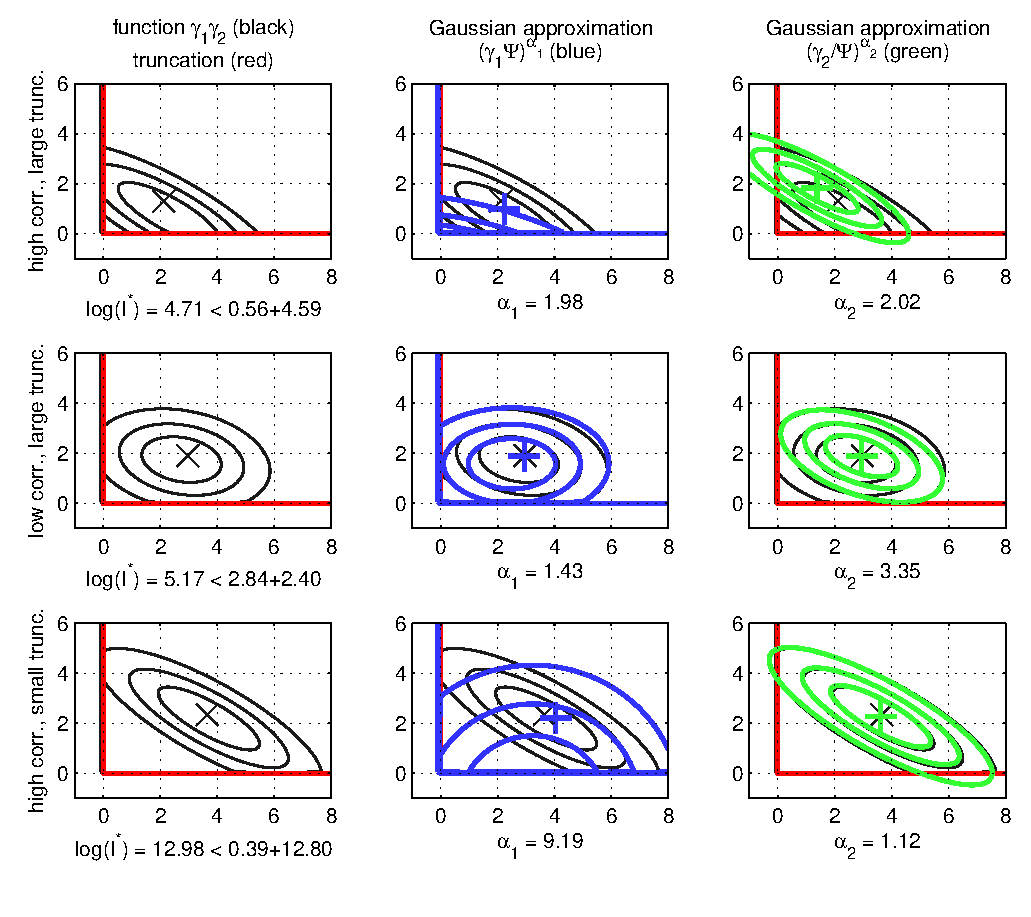
\includegraphics[width=.9\textwidth,, angle=0]{./pics/TruncGaussOrthant3_scissored.pdf}
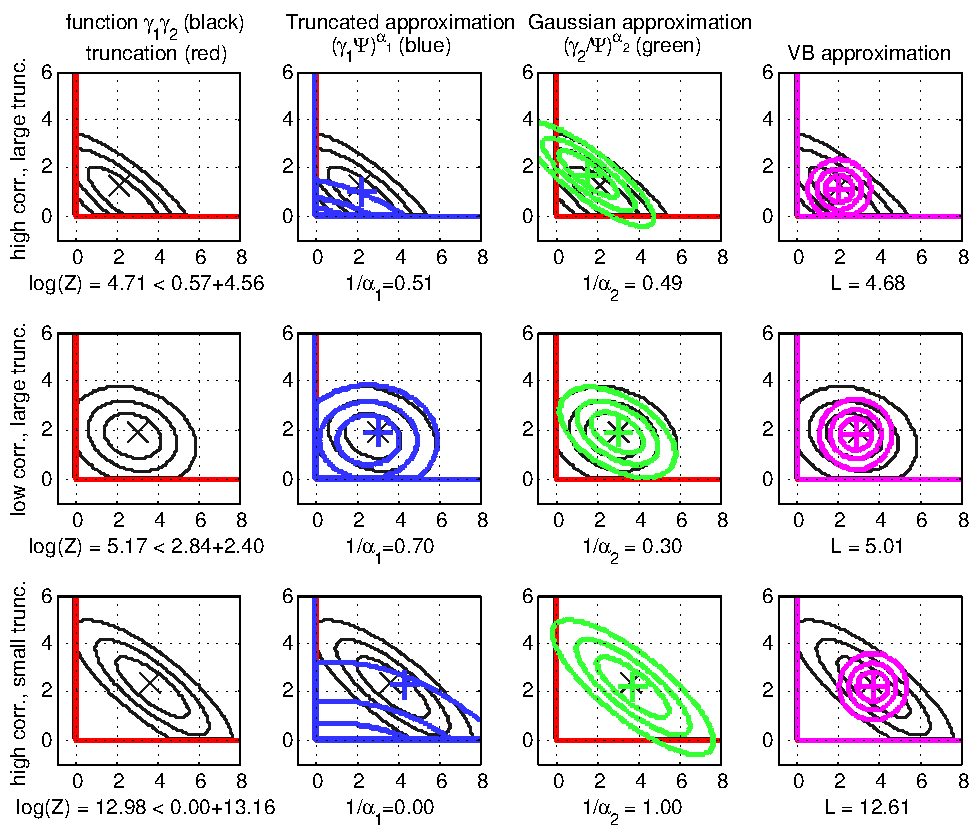
\includegraphics[width=.95\textwidth,, angle=0]{./pics/demo2d.pdf}
\vspace{-10pt}
%\vspace{-1.2cm}
\caption{2D Truncated Gaussian integration. Each row represents a different
correlation/truncation setting. From left to right, the columns show 
%1) the
%target function $fg$, 2) its first tractable approximation
%$f^{p}r^{\frac{1}{q}}$ (product of orthogonal univariate function) and 3)
%its second tractable approximation $g^{q}r^{-\frac{1}{p}}$ (correlated
%Gaussian distribution). 
1) the
target function $\gamma_1\gamma_2$, 2) its first tractable approximation
$(\gamma_1\Psi)^{\alpha_1}$ (product of orthogonal univariate function), 3)
its second tractable approximation $(\gamma_2/\Psi)^{\alpha_2}$ (correlated
Gaussian distribution) and 4) VB approximation. 
Symbols 'x' and '+' are the exact and approximate means, 
respectively.
}
\label{fig:TruncatedGauss}
\end{figure*}
%%%%%%%%%%%%%%%%%%%%%%%%%%%%%%%%%%%%%%%%%%%%%%


%%%%%%%%%%%%%%%%%%%%%%%%%%%%%%%%%%%%%%%%%%%%%%%%%%%%%%%%%%%%%%%%%%%%%%%%%%%%%%%%%%





\subsection{Truncated multi-variate Gaussian integration}
Most of the truncated multivariate Gaussian integration problems with linear
truncations can be put under the canonical form (\ref{univ-gaussian-integral})
where truncations are orthogonal,\footnote{ In their general form, truncated Gaussian integration problems
are based on the estimation of $\int_{\Re^n}  \prod_{i=1}^n f_i(\alpha_i +
\beta_i\transp t_i) e^{-\frac 12 \t\transp \A \t + b\transp \t} d\t$, but a
change of variable $\alpha_i + \beta_i\t_i \rightarrow \t_i$ leads to the
canonical form \eqref{univ-gaussian-integral} if there is no parallel truncation
lines, i.e. box constraints. Box constraints can be handled by a simple
modification involving two-sided univariate truncations. 
%See the Appendix~D for an example.
}
 i.e.
 $f_i(x)=\Indic{x\ge 0}$ for all $i\in\{1,\cdots,n\}$.
Integrating truncated correlated Gaussian is a known open problem for which
several approximation techniques have been proposed.
In numerical approximation,
adaptive quadratures approach have been well
investigated~\citep{genz2009computation}, but are still limited to small
dimensions. Approximate inference techniques,
such as Expectation-Propagation (EP), have been recently proposed, but the algorithm
remains unstable, even after specific improvements to increase the accuracy of
the method~\citep{Cunningham-et-al-Gaussian-EP2012}.
One of the reason is the fact that EP does not give any guarantee about the
approximation. To be used in a learning framework, upper and lower
bounds to the integral~(\ref{univ-gaussian-integral}) are often very useful. 
We focus here on the upper bound.\footnote{Lower bounding is not straightforward, since the
classical approach to obtain lower bounds is based on the information inequality
requires a class of approximation which is is contained in the support of the
target distribution, and this is not the case for multivariate Gaussian
distributions.} 
%
\paragraph{Initialization}
We need to initialize parameters so that the integral is tractable. This is not always trivial, but in principle, 
any point in the convex set $\tauspace=\{(\btau_1\transp, \btau_2\transp)\transp \in\Re^{2n} | 0\prec\diag{\btau_1}\prec A \}$ leads to a finite integral. For example, setting $\tau_{1i}$ to half of the minimum Eigen value of $A$ lies within the convex set.


\paragraph{Bound minimization}
After simplification, we get the following overall objective for the upper bound of a 
multivariate truncated Gaussian:
 \begin{flalign}
 \label{eq:obj}  
	%\frac 1{\alpha_1}  \sum_i  \log\Phi(\tau_{2i}\sqrt{\alpha_1/\tau_{1i}})  - n\mathcal{H}(\frac{1}{\alpha_1}) + C
	\frac 1{\alpha_1}  \sum_i  \log\unigint{f_i}(\tau_{1i},\tau_{2i}, \alpha_1)  
%\nonumber	 \\&&
%	 \quad
	 %+ \frac 1{\alpha_1} J(\frac 1{\alpha_1}\diag{\btau_1}, \tau_2)   
%	 \nonumber
%	 \\	 
  	 + \frac 1{\alpha_2} J({\alpha_2}(A-\diag{\btau_1}), {\alpha_2}(b-\tau_2))  + C
\end{flalign}

where $C:=-\frac n2 \log (2\pi)$. 
%We do not need to use a projection step in the gradient descent algorithm because the $\log-$determinant  functions act as barrier functions: they prevent the solution estimate to move outside the constraint set.\footnote{The objective function equals $\infty$ outside $\tauspace$.}

Figure~\ref{fig:TruncatedGauss} presents results on a two dimensional truncated gaussian integration problem. The optimal value of $\alpha_1$ depends on both the level of truncation and the correlation. %We observe that the mean of the tractable integrals provides a good approximation to the exact mean.


%%%%%%%%%%%%%%%%%%%%%%%%%%%%%%%%%%%%%%%%%%%%%%%%%%%%%%%%%%%%%%%%%%%%%%%%%%%%%%%%%%

\subsection{VB for truncated multi-variate Gaussian integration}
We start with \eqref{univ-gaussian-integral}: 
\begin{align}
\log I^*:=\log \int_{\Re^n}  \prod_{i=1}^n f_i(t_i)
e^{-\frac 12 \t\transp \A \t + \bm b\transp \t} d\t  \geq L
\end{align}
where $L$ denotes the negative variational free energy, a.k.a.~the variational lower bound, given by
\begin{align}
L := \sum_{i=1}^n \E{q}{\log f_i(t_i)}
-\frac 12  \trace(\A \E{q}{\t \t\transp}) + \bm b\transp \E{q}{\t}  + \entropy[q]
\end{align}
We choose the variational distribution $q$ to be a product of univariate truncated normal distributions which are truncated at zero. Let $q=\prod_i \truncnormdist(\mu_i, \sigma_i)$. The variational bound is given by
\begin{align}{
L &=  -\frac{1}{2}\trace(A \E{q}{\t\t\transp}) + \bm b\transp \E{q}{\t}  +\frac{n}{2}\log(2\pi e)  +\frac{1}{2}\sum_i\Bigl( \log\bigl(\sigma_i \Phi(\frac{\mu_i}{\sigma_i})\bigr) - \frac{\mu_i}{ \sqrt{2\pi} \sigma_i \Phi(\frac{\mu_i}{\sigma_i}) } \exp(-\frac{1}{2}\frac{\mu_i^2}{\sigma_i^2}) \Bigr), \nonumber\\
%elbo = -0.5*trace(params.A * E_tt) + params.b'*E_t +0.5*n*log(2*pi) +0.5*sum(log(sigma)) ...
%    +0.5*sum( sigma.^2 - mu .* sigma / sqrt(2*pi) .* exp(-0.5*(mu_over_sigma2)) ./ normcdf_mu_over_sigma);
%mu_over_sigma = mu ./ sigma;
%mu_over_sigma2 = mu_over_sigma.^2;
%normcdf_mu_over_sigma = normcdf(mu_over_sigma);
%
\E{q}{t_i} &= \mu_i + \frac{\sigma_i}{ \sqrt{2\pi} \Phi(\frac{\mu_i}{\sigma_i})}  \exp(-\frac{1}{2}\frac{\mu_i^2}{\sigma_i^2}),  \nonumber\\
\E{q}{t_i^2} &= \mu_i^2 + \sigma_i^2 + \frac{\mu_i\sigma_i}{ \sqrt{2\pi} \Phi(\frac{\mu_i}{\sigma_i})}  \exp(-\frac{1}{2}\frac{\mu_i^2}{\sigma_i^2}) 
\qquad \textnormal{and}\qquad \E{q}{t_i t_j} = \E{q}{t_i} \E{q}{t_j} \forall i\neq j.
}\end{align}

%%%%%%%%%%%%%%%%%%%%%%%%%%%%%%%%%%%%%%%%%%%%%%%%%%%%%%%%%%%%%%%%%

\subsection{Probit regression}
\label{probit}
%Probit regression is a GLM for binary observations.
In Bayesian statistics, probit regression is often preferred to logistic
regression as there is a natural interpretation of the model as a multivariate
truncated Gaussian variable, corresponding exactly to the integral 
studied in the previous section.
While efficient sampling and variational algorithms~\citep{opper2000gaussian, csato2002sparse} 
have been proposed, we show here that similar performances can be obtained using the 
variational \Holder approach. In brief, we apply the upper bounding technique to the evidence
integral to obtain tractable approximations.

Let $\dataset=(\X,\y)$, where $\X\in\Re^{m\times d}$ is the data matrix, i.e.
$X_{ij}$ is the value of the $j$-th covariate for the $i$-th data point, and
$\y\in\{-1,1\}^m$ the vector of binary output variables. We define $\Z$ as the
signed data matrix, such that $\Z_{ij} = y_i X_{ij}$.
With these notations, the likelihood function is:
$$ \proba(\dataset|\w) = \prod_{i=1}^m \proba(y_i|X_{i1},\cdots,X_{id},\w)  =
\Phi(\Z\w) \enspace, $$ where the function $\Phi:\Re^m\mapsto [0,1]$ 
is the product of normal CDFs:
\begin{align}
\Phi(\s)
% &=& 
= 
\prod_{i=1}^m \int_{-\infty}^{s_i} \normdist(u_i|0,1) du_i 
%\nonumber
%\\&=&
=
\int_{\Re^m}
\Indic{\v  \ge 0} \normdist(\v|\s,\eye_m) d\v \enspace,
\nonumber
\end{align}
 with
$\normdist(\u|\bm\mu,\Sigma)$ being the multivariate Gaussian PDF with mean $\bm\mu$ and
covariance matrix $\Sigma$.
\newcommand{\blambda}{\bm{\lambda}}
% =  (2\rho)^{-\frac{d}{2}} e^{-\frac 12 \|u\|^2}$ denotes the unit normal pdf.
We consider $d$-dimensional normal priors $\proba(\w|\blambda):=\normdist(\w| \bzeros_d,\diag{\blambda})$
where $\blambda\in (0,\infty)^d$.
%where $\bm\mu_0:Re^p\mapsto\Re^d$ and $\Lambda_0:\Re^p\mapsto\mathcal{S}_d^+$ are the prior mean and precision matrix 
%parameterized by the $p$-dimensional vector $\lambda$.
% 's parameterized by a common scale~$\lambda$:
% $\proba(\w):= c(\lambda)^{-d} \prod_{j=1}^d e^{-\frac{\lambda}{2} \ell(w_j)}$
% where $\ell$ is a univariate loss corresponding to the negative log-likelihood
% of a Student, Laplace or Gaussian distribution and $c$ is the partition
% function of the prior: $c(\lambda):=\int_\Re e^{-\frac{\lambda}{2}
% \ell(z)}dz$.
The marginal data probability (evidence) $\proba(\dataset|\lambda)$ is obtained by averaging this
likelihood over the prior distribution:

\begin{align}
\int_{\Re^d} \proba(\dataset|\w) d\proba(\w|\lambda)
%\\&=&
&=
\int_{\Re^d} \Phi(\Z\w) d\proba(\w)
% \nonumber\\
% && 
 =\int_{\Re^{d}}\int_{\Re^{+m}} %\Indic{\v \ge 0} 
 \normdist(\v|\Z\w,\eye_m) \normdist(\w|\bzeros_m,\diag{\blambda}) d\v d\w
\nonumber\\
&= c_\lambda \times \int_{\Re^{d+m}}e^{-\frac 12 \t\transp A_\lambda \t}  \prod_{i=1}^{n} f_i(t_i)  d\t
\label{prod-space}
\end{align}

with $n=d+m$, $c_\lambda = {(2\pi)^{-\frac{n}{2}}} {\prod_{i=1}^n\sqrt{\lambda_i}}$,
\begin{eqnarray} 
&&\A_\lambda = 	\left[\begin{array}{ll}
		 \diag{\blambda}  + \Z \transp \Z & -\Z\transp
		\\
		-\Z & \eye_m
	\end{array}
	\right]
	\\
&& \textrm{and}\quad\  f_i(t_i) =  	\left\lbrace\begin{array}{ll}
		1 &\ \textrm{if}\ i\le d \\
		\Indic{t_i\ge 0} &\ \textrm{otherwise} 
	\end{array}
	\right.
\enspace.
\end{eqnarray}
The symbols $\eye$ and $\bzeros$ denote the identity and zero matrices.
Equation~(\ref{prod-space}) is based on the concatenation $\t:=[\w\transp,\v\transp]\transp$ and 
corresponds exactly the same form as Equation~\eqref{univ-gaussian-integral}, i.e. a correlated Gaussian PDF multiplied by orthogonal $n=d+m$ univariate functions. 
We can now use the  VH bound on truncated correlated Gaussian model to obtain  an upper bound to the evidence, parameterized by $\btau$:
\begin{eqnarray} 
 \log \proba(\dataset|\lambda) \le  \log \overline{\proba}_\tau(\dataset|\lambda) 
\enspace.
\end{eqnarray}
The final approximation to the log-partition function is either a diagonal covariance Gaussian with truncation $(\gamma_1\Psi)^{\alpha_1}$ or a correlated Gaussian with no truncation $(\gamma_2/\Psi)^{\alpha_2}$.
The objective given by Equation~\eqref{eq:obj} becomes:
 \begin{flalign}
 \label{eq:obj-probit}  
%	&
	\frac 1{\alpha_1}  \sum_{i=d+1}^n  \log\Phi({\tau_{2i}}\sqrt{\frac{\alpha_1}{\tau_{1i}}})
%\nonumber	 \\
%	 \quad
%	& 
	-  \sum_{i=1}^n \frac 1{2\alpha_1}\log(\alpha_1\tau_{1i})  + \frac{\tau_{2i}^2}{2\tau_{1i}} 
%	 \nonumber
%	 \\	 
 % 	 &
	 + \frac 1{\alpha_2} J({\alpha_2}(A-\diag{\btau_1}), {\alpha_2}(b-\tau_2))  + C
\end{flalign}

\paragraph{Automatic model selection by maximizing the evidence}
Type II maximum likelihood, also called \emph{Empirical Bayes} method, is a simple way to choose the prior distribution: the data evidence given by Formula~(\ref{prod-space}) is maximized, with respect to the parameters $\lambda$ of the prior distribution.% For example, one usually chose $\bm\mu_0(\lambda):=\bzeros_{d\times 1}$ and $\Lambda_0(\lambda):=\lambda \eye_d$.
Since the variational \Holder inequality gives an approximation $\overline{\proba}_\tau(\dataset|\lambda)$ to the exact data evidence $\proba(\dataset|\lambda)$, one can choose the best of these approximations, i.e. the one minimizing the upper bound. Maximizing the minimal upper bound corresponds to a max-min problem:
\begin{eqnarray} 
\max_{\lambda\in\Re^+} \min_{\tau\in\tauspace} \log \overline{\proba}_\tau(\dataset|\bzeros,\diag{\blambda})
\enspace.
\end{eqnarray}
\red{The objective function $ \log \overline{\proba}_\tau(\dataset|\bzeros,\diag{\blambda})$ being concave in $\lambda$ and convex in $\tau$, this is a well defined saddle point problem. A solution can be found using standard tools from convex optimization, such as the Arrow-Hurwicz-Uzawa algorithm~\citep{arrow1958studies, nedic2009subgradient}.}

%Note that the loss $\ell$ is not necessarily convex, but the variational inference problem is convex. 



%\clearpage
\section{Experiments}
To illustrate how the bound is applied in practice, we focus on a toy example.
We use a 1-dimensional toy probit regression example. We set $N=2$ and $\bx_1=1, \bx_2=-1$ and $y_1=1, y_2=-1$. For simplicity, we fix the prior over $w$ to $\normdist(0,1)$ and run the classic augmented variable Gibbs sampler proposed by \citet{albert1993bayesian} for 5000 iterations. We plot the running mean of posterior samples of $w$ as a function of the iteration. We repeat this procedure 100 times. The running mean for multiple iterations is shown in Fig.~\ref{fig:albertchib}. 
We observe that the running mean converges after 2000 iterations in all runs, indicating the convergence of the sampler. The average of the running mean (after convergence) over multiple runs is 0.8477 and the $90\%$ quantile is given by $[0.8204, 0.8769]$.  We use this as ground truth to evaluate the quality of the solution from VH.

%\begin{figure}[htbp]
%\begin{center}
%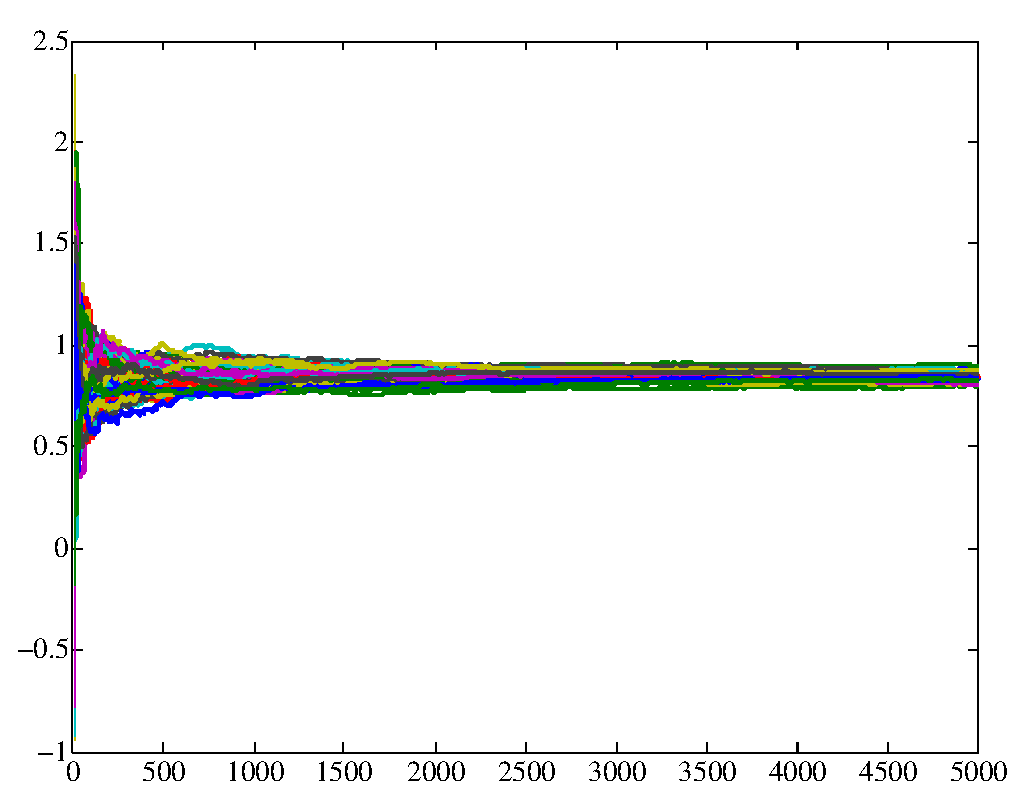
\includegraphics[scale=0.45]{../../src/VariationalHolder/matlab/blogreg/ProbRegSamp/albertchib}
%\caption{Running mean of  samples drawn from the posterior over $w$ as a function of iteration. The plot shows 100 repetitions of the procedure.}
%\label{fig:albertchib}
%\end{center}
%\end{figure}

We used the {SciPy} implementation of modified Powell's method\footnote{\url{http://docs.scipy.org/doc/scipy-0.14.0/reference/generated/scipy.optimize.fmin_powell.html}.} to minimize the VH bound in Equation~\eqref{eq:obj-probit}.  We compute moments of each of the integrals and compute the overall moments as follows:
$\bar\w_{1i} = \int \z (\gamma_1(\z_i)\Psi(\bz;\hat\tau))^{\alpha_1}d\nu(\bz)/\|\gamma_1(\z_i)\Psi(\bz;\hat\tau)\|^{\alpha_1}_{\alpha_1}$ corresponds to a
truncated Gaussian expectation and $\bar\w_{2i} = \int \z (\gamma_2(\z_i)/\Psi(\bz;\hat\tau))^{\alpha_2}d\nu(\bz)/\|\gamma_2(\z_i)\Psi(\bz;\hat\tau)\|^{\alpha_2}_{\alpha_2}$
is just the mean of a Gaussian distribution.
%$\Expectation{$
The moments computed using VH were $\bar\w_{1}=0.807, \bar\w_{2}=0.822$ and the convex combination was $\bar\w_{12}=0.8146$. %with $\alpha_1=2$. 
We observe that even though there is a slight bias, the VH solution is very close to the solution obtained via sampling. %by the Albert and Chib sampler.

%\begin{table}[htdp]
%\caption{Results on toy 1 dimensional dataset}
%\begin{center}
%\begin{tabular}{|c|c|c|c|}
%% $\dfrac{1}{\alpha_1}$
%\hline
%$\rho$ & $1/\alpha_1$ & VH & Gibbs $90\%$ interval \\
%\hline
%0.1 & 0.875 & -0.4 & (0.7, 0.72)  \\
%0.25 &  0.868 & -1.48 &  (1.31, 1.35)  \\
%0.5 & 0.869 & 2.09& (2.29, 2.43) \\
%1 & 0.834 & 3.97 & (3.55, 3.59) \\
%3 & 0.781 & 4.81& (4.8, 4.82) \\
%10 & 0.769 &4.97 & (5.04, 5.07) \\
%\hline
%\end{tabular}
%\end{center}
%\label{tab:toy1d}
%\end{table}%

Next, we use $N=100$ data points and generate training data as follows: $x_m\sim \normdist(\rho y_m,1)$. The higher $\rho$, the more separable the two classes are. The values of the moments are shown in Table~\ref{tab:toy1dall}. We observe that as the $\rho$ increases, the problem simplifies and the optimal value of $1/\alpha_1$ increases implying that the overall posterior is `more Gaussian'.

\begin{table}[htdp]

\begin{center}
\resizebox{0.55\columnwidth}{!}{
\begin{tabular}{|c|c|c|c|c|c|}
% $\dfrac{1}{\alpha_1}$
\hline
$\rho$ & $1/\alpha_1$ & $\bar\w_{1}$ & $\bar\w_{2}$ & $\bar\w_{12}$ (mix) & Gibbs $90\%$ CI \\
\hline
%0.1 & 0.875 & -0.575 & 0.82 & -0.4 & (0.7, 0.72)  \\
%0.25 &  0.868 & -1.89 & 1.23 & -1.48 &  (1.31, 1.35)  \\
0.5 & 0.869 & 2.03 & 2.54 & 2.09& (2.29, 2.43) \\
1 & 0.834 & 4.05 & 3.56 & 3.97 & (3.55, 3.59) \\
3 & 0.781 & 4.77 & 4.92  & 4.81& (4.8, 4.82) \\
10 & 0.769 & 4.93 & 5.1 & 4.97 & (5.04, 5.07) \\
\hline
\end{tabular}
}
\end{center}
\caption{Results on one dimensional dataset.}% for varying $\rho$.}
\label{tab:toy1dall}
\end{table}%

%\begin{table}[htdp]
%\caption{Results on toy 2 dimensional dataset}
%\begin{center}
%\begin{tabular}{|c|c|c|c|}
%% $\dfrac{1}{\alpha_1}$
%\hline
%$\rho$ & $1/\alpha_1$ & VH & Gibbs \\
%\hline
%0.1 & 0.856 & 0.83, 0.83 & -0.04, 0.04  \\
%0.5 & 0.814 & 2.51, 2.44 &  1.2, 2.14 \\
%1 & 0.786 &  3.25, 3.25 & 3.05, 3.07  \\
%3 & 0.766 & 3.32, 3.58 & 3.53, 3.52 \\
%10 & 0.758 & 3.53, 3.66 &  3.55, 3.63 \\
%\hline
%\end{tabular}
%\end{center}
%\label{tab:toy2d}
%\end{table}%


%
%\subsection{Toy problem with tractable solutions}
%Start with problems where integral is analytically tractable (e.g. conjugate exponential families) and compare VH solution with true solution
%
%
%\subsubsection{Product of probits - Solution 1}
%We want to compute the unidimensional integral of $\gamma(x):=e^{-\frac{\lambda_0}{2} x^2}\Phi(a_1 x + b_1)\Phi(a_2 x + b_2)$,
%where $\Phi$ is the Gaussian cdf $\Phi(t) := (2\pi)^{-\frac 12}\int_{-\infty}^t e^{-\frac{z^2}{2}} dz$.
%
%We know how to integrate the product of a Gaussian pdf and a Gaussian cdf:
%\begin{eqnarray}
%	\int_\Re \Phi(a x + b) e^{-\frac{c}{2} x^2}  dx = \frac{1}{c} \Psi\left( \frac{b}{\sqrt{a^2 + 1}}\right)
%	\enspace.
%\end{eqnarray}
%and more generally we define the special function $S:\Re^4\mapsto \Re$ as:
%\begin{eqnarray}
%	S(a,b,c,\delta) := \int_\Re \Phi(a x + b) e^{-\frac{c}{2} x^2 + \delta x} dx = \frac{1}{c} e^{\frac{\alpha^2}{2c}} \Psi\left( \frac{b + \frac{a d}{c}}{\sqrt{a^2 + 1}}\right)
%	\enspace.
%\end{eqnarray}
%So, if the pivot function has a squared-exponential shape, i.e. $\Psi(x):=e^{-\tau_1 \frac{x^2}{2} + \tau_2}$ we can choose:
%\begin{itemize}
%\item $\gamma_1(x):=\Phi(a_1 x + b_1) e^{-\frac 12 \tau_1 x^2 + \tau_2 x}$
%\item $\gamma_2(x):=\Phi(a_2 x + b_2) e^{-\frac 12 (\lambda_0-\tau_1) x^2 - \tau_2 x}$
%\end{itemize}
%One can check that $\gamma=\gamma_1\gamma_2$. To be able to integrate theses functions, we need that $0<\tau_1<\lambda_0$, and we get:
%\begin{itemize}
%\item $\int_\Re\gamma_1(x) dx = S(a_1, b_1, \tau_1, \tau_1)$
%\item $\int_\Re\gamma_2(x) dx = S(a_2, b_2, \lambda_0 - \tau_1, -\tau_2)$
%\end{itemize}


%\subsection{VH vs sampling for Bayesian logistic regression}
%\begin{itemize}{
%\item VH is convex optimization problem, however it's not clear if the VH minima corresponds to a useful solution for the true posterior
%\item Gibbs sampling: hard to assess convergence
%}\end{itemize}
%
%
%\subsection{VH vs VB}
%\begin{itemize}{
%\item Experiment that illustrates advantage of global optima of VH over local optima of VB
%\item \red{BL: I think it'd be interesting to compare VH and VB on a problem where the target distribution has subspaces with zero probability.}
%}\end{itemize}
%

%\section{Prior art}




\section{Generalization for many factors}
\label{many-factor}
In the previous section, we showed that probit regression can be interpreted as the product of two tractable functions. In this 
section, we consider the more general case where the integral to compute is the product of $K$ factors, $K>2$:
$\I^*:=\int \prod_{k'=1}^K f_k(\z) d\basem(\z)$ where $f_k$, $k=1,\cdots, K$ are the individual factors.
%Let us define a non-negative pivot function as the product of per-potential pivot function $\Psi(\t):=\prod_{k=1}^K \Psi_k(\t)$. 
We have the following results:
\begin{theorem}
The following inequality:
%{\small
\begin{eqnarray}
\label{eq:generalization}
I^*
&\le& 
\prod_{k=1}^K \left(
	\int_{\Zspace} {\left(\frac{f_k(\z)}{\Psi_k(\z)}\right)}^{\alpha_k} 
	\prod_{k'=1}^K \Psi_{k'}(\z) d\basem(\z)
	\right)^{\frac{1}{\alpha_k}}
\label{eq:Holder2}
\end{eqnarray}
%}
holds for any $\balpha=(\alpha_1,\cdots,\alpha_K)\in(0,\infty)^K$ such that $\sum_{k=1}^K \frac{1}{\alpha_k}=1$
and any function $\Psi_k:\Zspace\mapsto\Re^+$ in $\mathcal{L}_{\alpha_k}$, $k=1,\cdots, K$.
\end{theorem}
\begin{proof}(sketch)
Similarly to the generalization of \Holder's inequality for a product of functions, we can apply the binary VH bound recursively.
\end{proof}\\
One can verify that we recover the results of Section~2 for $K=2$. 
The VH method can be obtained by parameterizing the pivot functions and minimizing~\eqref{eq:generalization}  with respect
to the pivot functions $\Psi_k$ and $\balpha$.
Tightness and approximation properties studied in Section~3
can also be extended to the case of multiple factors.

%\section{VARIATIONAL HOLDER VS.~VARIATIONAL BAYES}
\section{Variational \Holder vs.~Variational Bayes}
One can compare the VH inequality~(\ref{eq:VH-logspace}) to the one provided by the \emph{Variational Bayes} 
(VB) inequality:
\begin{align}
\log\I^*
\ge 
\int \log\gamma_1(\z) dq(\z) + 
\int \log\gamma_2(\z) dq(\z) +
\mathcal{H}(Q)
\enspace.
\label{eq:VB-logspace}
\end{align}
for any distribution $Q$ absolutely continuous with respect to $\nu$, where $\mathcal{H}$ denotes the information entropy and $q=\frac{dQ}{d\nu}$. 

VB provides a lower bound to the log-sum-exp function, while the VH provides an upper bound. One disadvantage
 of the VB bound~(\ref{eq:VB-logspace}) is that it is not concave in general, 
leading to objective functions that are difficult to maximize and a bound that
does not come with theoretical guarantees. Another disadvantage is that the approximating
distribution $Q$ must have a support included in the base distribution $\nu$, which is not 
always convenient when the target distribution has subspaces with zero probability. 
This \emph{zero-avoiding} effect of the VB bound can lead to 
crude approximations of the original integral~\citep{minka2005divergence}.
%e.g. when distributions have zero probability on some subsets of the space.



%%%%%%%%%%%%%%%%%%%%%%%%%%%%%%%%%%%%%%%%%%%%%%%%%%%%%%%%%%%%
\section{Discussion}
We have introduced a new family of variational approximations that are based on the 
minimization of an upper bound to the log-partition function. We demonstrated that
the variational inference problem is convex if the variational function is log-linear, 
which has great practical and theoretical advantages over mean-field/VB approximations,
which is the main approach used today by practitioners. We also provide a novel way to
handle sparse regression in GLMs. In fact, we focused on probit regression, but the extension to
other losses is easy. One of the unique feature of this approach is that
the sparse factors might be heavy tails, but we still maintaining
a convex objective. Further experiments will be conducted to evaluate how good this 
approximation behaves in very sparse models. 

The VH framework presented here is very general, and can be applied to many models and
optimized using a large variety of algorithms and speedup tricks, similarly to what happened 
with VB and EP other the last two decades. 
%An interesting line of work would be optimize the VH bound using stochastic gradient methods.

We focused mainly on one type of intractable integrals that is common in machine learning 
problems (GLM or linear models with sparse priors), but the approach is generic and
could potentially be applied in many other settings. One of the main area of application
is the inference in graphical models with discrete variables, on which the TRW sum-product
algorithm has been designed~\citep{wainwright2005new}, as well as several other
algorithms dedicated to discrete graphical models~ \citep{liu11d}. It also provides an upper bound to the log-partition function
and is convex if the tree-weights are known. An alternative proof to the TRW bound based on the \Holder inequality
was given by~\citet{minka2005divergence}, and we conjecture that the TRW bound could be 
expressed as a special case of the proposed approach, for example by assuming that there is 
one factor per possible spanning tree.


%\subsection{Citations and References} 

\newpage
\bibliography{holder}
\bibliographystyle{plainnat}





\renewcommand{\f}{f}
\renewcommand{\g}{g}
\renewcommand{\p}{p}
\renewcommand{\q}{q}

%%%%%%%%%%%%%%%%%%%%%%%%%%%%%
%%%%%%%%%%%%%%%%%%%%%%%%%%%%%
%%%%%%%%%%%%%%%%%%%%%%%%%%%%%
\newpage
\vspace{-0.1in}
\section*{Appendix}
\vspace{-0.1in}
\subsection*{Pre-requisites}
In the following, the symbols $\f$ and $\g$ represent $\nu-$measurable positive functions, and $\p$ and $\q$ are positive  scalars such that $\frac 1\p+\frac 1\q=1$.


%%%%%%%%%%%%%%%%%%%%%%%%%%%%%
\vspace{-0.1in}
\begin{lemma}  
\label{lem:approx0}
For any $\varepsilon>0$, the inequality $\|\f\g\|_1> (1-\varepsilon) \|\f\|_\p \|\g\|_\q$ implies that:
\begin{align}
\left\|
	\frac{\f^{\p}}{\|\f\|^{\p}_{\p}} 
	- 
	%\frac{\f\g}{\|\f\|_{\p}\|\g\|_{\q}} 
	\frac{\f\g}{\|\f\|_\p \|\g\|_\q} 
\right\|_1 \le \sqrt{2\varepsilon}
\quad &  \mathrm{if} \quad \p \le 2, \mathrm{\ and}
%\label{eq:gbigger}
\nonumber
\\
\left\|
	\frac{\g^{\q}}{\|\g\|^{\q}_{\q}} 
	- 
	%\frac{\f\g}{\|\f\|_{\p}\|\g\|_{\q}} 
	\frac{\f\g}{\|\f\|_\p \|\g\|_\q} 
\right\|_1 \le \sqrt{2\varepsilon} 
\quad  & \mathrm{\ if \ } \p\ge 2
\label{eq:fbigger}
\end{align}
\end{lemma} 

\vspace{-0.1in}
%%%

\begin{proof}
Let assume that  $\|\f\|_{\p} \le \|\g\|_{\q}$ and $p\in(1,2]$. 
\begin{eqnarray}
&&
\left\|
	\frac{\f^{\p}}{\|\f\|^{\p}_{\p}} 
	- 
	%\frac{\f\g}{\|\f\|_{\p}\|\g\|_{\q}} 
	\frac{\f\g}{\|\f\|_\p \|\g\|_\q} 
\right\|_1
\nonumber\\
 &&= 
\left\|
	\frac{\f^{\frac{\p}{2}}}{\|\f\|^{\frac{\p}{2}}_{\p}} \left(\frac{\f^{\frac{\p}{2}}}{\|\f\|^{\frac{\p}{2}}_{\p}}
	- 
	%\frac{\f\g}{\|\f\|_{\p}\|\g\|_{\q}} 
	\frac{\f^{1-\frac{\p}{2}}\g}{\|\f\|^{1-\frac{\p}{2}}_\p \|\g\|_\q} 
	 \right)
\right\|_1 
\nonumber\\
&&\le
\underbrace{
\left\|
	\frac{\f^{\frac{\p}{2}}}{\|\f\|^{\frac{\p}{2}}_{\p}} 
\right\|_2
}_{=1}
\left\|	
	\frac{\f^{\frac{\p}{2}}}{\|\f\|^{\frac{\p}{2}}_{\p}}
	- 
	%\frac{\f\g}{\|\f\|_{\p}\|\g\|_{\q}} 
	\frac{\f^{1-\frac{\p}{2}}\g}{\|\f\|^{1-\frac{\p}{2}}_\p \|\g\|_\q} 
\right\|_2 
\label{eq:temp1}
\nonumber
\end{eqnarray}
by Cauchy-Schwartz inequality. We can expand the square of the right-hand term in the product:
\begin{eqnarray}
&&\left\|	
	\frac{\f^{\frac{\p}{2}}}{\|\f\|^{\frac{\p}{2}}_{\p}}
	- 
	%\frac{\f\g}{\|\f\|_{\p}\|\g\|_{\q}} 
	\frac{\f^{1-\frac{\p}{2}}\g}{\|\f\|^{1-\frac{\p}{2}}_\p \|\g\|_\q} 
\right\|_2^2 
\nonumber\\
&&= 
\underbrace{
\left\|	
	\frac{\f^{\frac{\p}{2}}}{\|\f\|^{\frac{\p}{2}}_{\p}}
\right\|_2^2
}_{=1}
- 2 
\underbrace{
\frac{\|fg\|_1}{\|\f\|_\p \|\g\|_\q}
}_{\ge 1-\varepsilon}
+ 
\underbrace{
\left\|	
	\frac{\f^{1-\frac{\p}{2}}\g}{\|\f\|^{1-\frac{\p}{2}}_\p \|\g\|_\q} 
\right\|_2^2
}_{:=A}
\nonumber
\\
&&\le A - 1 + 2\varepsilon
\label{eq:temp2}
\enspace,
\end{eqnarray}
where we denote by $A$ the quantity:
\begin{eqnarray}
A := \left\|	
	\frac{\f^{1-\frac{\p}{2}}\g}{\|\f\|^{1-\frac{\p}{2}}_\p \|\g\|_\q} 
\right\|_2^2
=\frac{\left\|	\f^{1-\frac{\p}{2}}\g \right\|_2^2}{\|\f\|^{2-\p}_\p \|\g\|_\q^2} 
=
	\frac{\left\|	\f^{2-\p}\g^2 \right\|_1}{\|\f\|^{2-\p}_\p \|\g\|_\q^2} 
\nonumber
\end{eqnarray}
Assuming $\p\le 2$, we can now bound $A$ by using \Holder's inequality with exponents $p'=\frac{\p}{2-\p}$ and $\q'=\frac{\q}{2}$. One can verify that the pair $(p',q')$ is a valid \Holder's exponent: $\q'\ge 1$, $\p'\ge1$ and $\frac{1}{\p'}+\frac{1}{\q'}=\frac{2-\p}{\p} + \frac{2}{\q} = \frac{2}{\p} +\frac{2}{\q} - 1 = 2-1=1$. We obtain:
\begin{eqnarray}
A &\le&
	\frac{\left\|	\f^{2-\p} \right\|_{\p'} \left\|\g^2 \right\|_{\q'} }
		{\|\f\|^{2-\p}_\p \|\g\|_\q^2} 
	=
	\frac{\left\|	\f \right\|_{\p}^{2-\p} \left\|\g \right\|_{\q}^2 }
		{\|\f\|^{2-\p}_\p \|\g\|_\q^2}  = 1
\nonumber
\end{eqnarray}
This results proves that Equation~\eqref{eq:temp2} is upper bounded by $2\varepsilon$, so the Equation~\eqref{eq:temp1} leads to the following inequality:
\begin{eqnarray}
\left\|
	\frac{\f^{\p}}{\|\f\|^{\p}_{\p}} 
	- 
	%\frac{\f\g}{\|\f\|_{\p}\|\g\|_{\q}} 
	\frac{\f\g}{\|\f\|_\p \|\g\|_\q} 
\right\|_1 &\le& 
\sqrt{2\varepsilon}
\label{eq:final}
\end{eqnarray}
Equation~\eqref{eq:fbigger} follows by symmetry. 
\end{proof}









%%%%%%%%%%%%%%%%%%%%%%%%%%%%%


\begin{theorem}  
\label{th:approx0}
For any $\varepsilon>0$, the inequality $\|\f\g\|_1> (1-\varepsilon) \|\f\|_\p \|\g\|_\q$ implies that:
\begin{align}
\left\|
	\frac{\f^{\p}}{\|\f\|^{\p}_{\p}} 
	- 
	%\frac{\f\g}{\|\f\|_{\p}\|\g\|_{\q}} 
	\frac{\f\g}{\|\f\g\|_1} 
\right\|_1 \le \sqrt{2\varepsilon} + \varepsilon
\quad &  \mathrm{if} \quad \q\ge\p, \mathrm{\ and}
\nonumber
\\
\left\|
	\frac{\g^{\q}}{\|\g\|^{\q}_{\q}} 
	- 
	%\frac{\f\g}{\|\f\|_{\p}\|\g\|_{\q}} 
	\frac{\f\g}{\|\f\g\|_1} 
\right\|_1 \le \sqrt{2\varepsilon} + \varepsilon
\quad  & \mathrm{\ if \ } \quad \p\ge\q
\label{eq:fbigger2}
\end{align}
\end{theorem} 


%%

\begin{proof}
\begin{eqnarray}
&&\left\|
	\frac{\f^{\p}}{\|\f\|^{\p}_{\p}} 
	- 
	%\frac{\f\g}{\|\f\|_{\p}\|\g\|_{\q}} 
	\frac{\f\g}{\|\f\g\|_1} 
\right\|_1
\nonumber\\
&&
\le 
\underbrace{
\left\|
	\frac{\f^{\p}}{\|\f\|^{\p}_{\p}} 
	- 
	%\frac{\f\g}{\|\f\|_{\p}\|\g\|_{\q}} 
	\frac{\f\g}{\|\f\|_\p \|\g\|_\q} 
\right\|_1
}_{\le\sqrt{2\varepsilon}\ \mathrm{by~Lemma~\ref{lem:approx0} }}
+
\underbrace{
\left\|
	\frac{\f\g}{\|\f\|_\p \|\g\|_\q} 
	- 
	%\frac{\f\g}{\|\f\|_{\p}\|\g\|_{\q}} 
	\frac{\f\g}{\|\f\g\|_1} 
\right\|_1
}_{\le \varepsilon}
\nonumber
\end{eqnarray}
Equation~\eqref{eq:fbigger2} follows by symmetry.
\end{proof}

%
%\begin{theorem}  
%\label{th:approx0}
%There exists finite constants $C_1$ and $C_2$ such that for any $\varepsilon>0$, the inequality $\|\f\g\|_1> (1-\varepsilon) \|\f\|_\p \|\g\|_\q$ implies that:
%\begin{align}
%\left\|
%	\frac{\f^{\p}}{\|\f\|^{\p}_{\p}} 
%	- 
%	%\frac{\f\g}{\|\f\|_{\p}\|\g\|_{\q}} 
%	\frac{\f\g}{\|\f\g\|_1} 
%\right\|_2 \le C_1 \sqrt{\varepsilon} + \varepsilon
%\quad &  \mathrm{if} \quad \|\f\|_{\p} \le \|\g\|_{\q}, \mathrm{\ and}
%\label{eq:gbigger}
%\\
%\left\|
%	\frac{\g^{\q}}{\|\g\|^{\q}_{\q}} 
%	- 
%	%\frac{\f\g}{\|\f\|_{\p}\|\g\|_{\q}} 
%	\frac{\f\g}{\|\f\g\|_1} 
%\right\|_2 \le C_2 \sqrt{\varepsilon} + \varepsilon
%\quad  & \mathrm{\ if \ } \|\f\|_{\p} \ge \|\g\|_{\q}
%\label{eq:fbigger}
%\end{align}
%\end{theorem} 
%
%\begin{proof}
%Let assume that  $\|\f\|_{\p} \le \|\g\|_{\q}$. 
%
%
%Equation~\eqref{eq:fbigger} follows by symmetry.
%\end{proof}
%


\subsection*{Proof of Proposition~\ref{th:approx}}
We are now ready to obtain the proof for the bound approximation property:

\begin{proof}
Apply Theorem~\ref{th:approx0} with $f:=\gamma_1\Psi$, $\g:=\gamma_2/\Psi$, $\p:=\alpha_1$, $\q:=\alpha_2$, $I^*:=\|\f\g\|_1$ and $\bar I_\balpha (\Psi):= \|\gamma_1\Psi\|_\p\|\gamma_2/\Psi\|_\q$.
\end{proof}







%%%%%%%%%%%%%%%%%%%%%%%%%%%%%%%%%%%%%%%%%%%%%%%%%%%%%%%%%%%%%%%%%%%%%%



%
%\section{Efficient minimization of the objective function}
%To minimize the function \eqref{eq:obj}, we first upper bound the $\log\Phi$ term by a quadratic function by using a Taylors approximation at points $\eta_i$ and the fact that $\nabla^2\log\Phi\le1$.
%Let define $\breve{I}(\tau,\eta)$ as:
%{\small
% \begin{eqnarray}  
%  \label{eq:obj-ub}  
%&&	  a +  \sum_i b_i (\tau_{2i}\sqrt{\alpha_1/\tau_{1i}}-\eta_i) +  c_i(\tau_{2i}\sqrt{\alpha_1/\tau_{1i}}-\eta_i)^2
%	 \nonumber\\&&
%	 - \frac 1{2\alpha_1} \log|\diag{\btau_1}|   - \frac 1{2\alpha_2} \log|A-\diag{\btau_1}|  
%	 \\&&
%	 + \frac{1}{2}\left ((b - \btau_2)\transp  (A-\diag{\btau_1})^{-1} (b - \btau_2) +\sum_i \tau_{2i}^2/\tau_{1i}\right)
%	 \nonumber
%\end{eqnarray}
%}
%where $a:=\frac 1{\alpha_1} \sum_i \log\Phi(\eta_i)  - n\mathcal{H}(\frac{1}{\alpha_1}) + C$, $b_i:=...$ and $c_i:=...$.
%We can minimize with respect to $\tau_2$ by identifying the quadratic form and obtain the solution:
%$\hat\btau_{2} := M^{-1} L$ where:
%{\small
% \begin{eqnarray}  
% &&
% M := (A-\diag{\btau_1})^{-1} +  \diag{\btau_1}^{-1} 
% 	 \nonumber\\&&
%\quad
%	+ 2 \diag{\{c_i\sqrt{\alpha_1/\tau_{1i}}\}_i}
%	 \\&&
%L:= ...
%\end{eqnarray}
%}
%For $\btau_1$, there is no closed for solution. 
%


%%%%%%%%%%%%%%%%%%%%%%%%%%%%%%%%%%%%%%%%%%%%%%%%%%%%%%%%%%%%%%%%%%%%%%








\end{document} 
%%%%%%%%%%%%%%%%%%%%%%%%%%%%%%%%%%%%%%%%%%%%%%%%%%%%%%%%%%%%%%%%%%%%%%
%%%%%%%%%%%%%%%%%%%%%%%%%%%%%%%%%%%%%%%%%%%%%%%%%%%%%%%%%%%%%%%%%%%%%%
%%%%%%%%%%%%%%%%%%%%%%%%%%%%%%%%%%%%%%%%%%%%%%%%%%%%%%%%%%%%%%%%%%%%%%
%%%%%%%%%%%%%%%%%%%%%%%%%%%%%%%%%%%%%%%%%%%%%%%%%%%%%%%%%%%%%%%%%%%%%%
%%%%%%%%%%%%%%%%%%%%%%%%%%%%%%%%%%%%%%%%%%%%%%%%%%%%%%%%%%%%%%%%%%%%%%





%%%%%%%%%%%%%%%%%%%%%%%%%%%%%%%%%%%%%%%%%%%%%%%%%%%%%%%%%%%%%%%%%%%%%%
\clearpage

\section{Bayesian Logistic Regression}
\label{sec:logreg}

Let $\bX\in\Re^{N\times D}$ a design matrix\footnote{The matrix $X$ contains features, possibly including a constant non-zero feature if the model includes an intercept parameter.} with rows\footnote{We will assume all the vectors (e.g. $x, \bbeta$) are column vectors.} $\bx_1\transp,\ldots, \bx_N\transp$ in $\Re^D$ and $\y\in\{-1,1\}^N$ the target values of a linear logistic regression model. Let $\D=\{\bX, \y\}$. 
Denoting by $\bbeta\in\Re^D$ the vector of parameters, the likelihood is:
$$ p(\y|\bbeta, \bX) = \prod_{n=1}^N \sigma(y_n \bx_n\transp \bbeta)$$
where  $\sigma:\Re\mapsto [0,1]$ % $\sigma:\Re\mapsto \Re$
 is the sigmoid $\sigma(\phi):=\frac{1}{1+e^{-\phi}}$.
Using a Gaussian prior $\normdist(\bbeta|\mu_0, \Sigma_0)$ we want to approximate the posterior over $\bbeta$:
\begin{align}
\label{eq:posterior}
 p(\bbeta|\D) \propto \normdist(\bbeta|\mu_0, \Sigma_0) \prod_{n=1}^N \sigma(y_n \bx_n\transp \bbeta).
\end{align}
 
\section{Polya-Gamma distribution}
\label{sec:pg}
The Polya-Gamma distribution is a two-parameter univariate distribution.  
%that can recover the sigmoid likelihood when marginalized.
\citet{polson2013bayesian} showed that the sigmoid function can be represented 
as a mixture of Gaussians with respect to a Polya-Gamma distribution.  
%The core inequality is:
%\begin{align}
%\label{eq:pg}
%\sigma(\phi) = \frac 12 e^{\frac{\phi}{2}} \int_{0}^{\infty} e^{-\omega\phi^2}\PG(\omega|1,0)d\omega,
%\end{align}
More precisely,  the sigmoid likelihood can be written as
\begin{align}
\label{eq:pg}
\sigma(\phi) = \frac{1}{2} e^{\frac{\phi}{2}} \int_{0}^{\infty} e^{-\frac{\omega}{2}\phi^2}\PG(\omega|1,0)d\omega,
\end{align}
where $\phi=y\bx\transp\bbeta$ and $\PG(\omega|1,0)$%$\PG(\omega|a,b)$ denotes the %is the pdf of $\PG(a,b)$, 
the Polya-Gamma distribution with parameters 1 and 0. %\red{scale parameter 1 and shift parameter 0}. 
{BL: I think the second parameter is the scale parameter ... not sure if the first parameter has an interpretation .. maybe we can call it the shape parameter?}  We refer the reader to \citep{polson2013bayesian} for further details about the Polya Gamma distribution.

%It was recently used to drastically speedup the sampling of Bayesian logistic regression through a data-augmentation~\citep{polson2013bayesian}.
\citet{polson2013bayesian} recently proposed a data-augmentation strategy for Bayesian logistic regression. The trick is to introduce auxiliary variables $\bomega=(\omega_1,\ldots,\omega_N)$ and use Gibbs sampling on the  augmented space; $\bbeta|\D,\bomega$ is a Gaussian  distribution, whereas $\bomega|\D,\bbeta$ is distributed according to a Polya-Gamma distribution. \citet{polson2013bayesian} present a strategy to sample from $\bomega|\D,\bbeta$, however the Gibbs sampling strategy might suffer from mixing issues. We will discuss a different strategy to compute the posterior in \eqref{eq:posterior}.
%We will use the same idea to derive our posterior.


\section{Bayesian Learning of Logistic Regression}
\label{sec:blr}
Plugging in Equation~\eqref{eq:pg} into Equation~\eqref{eq:posterior}, the posterior $p(\bbeta|\mathcal{D})$ is proportional to:
\begin{align}
\label{eq:posterior2}
\normdist(\bbeta|\mu_0, \Sigma_0) e^{\frac{1}{2}\y\transp X \bbeta} \prod_{n=1}^N \int_{0}^{\infty} e^{-\frac{\omega_n}{2} (\bx_n\transp \bbeta)^2} \PG(\omega_n|1,0)d\omega_n
\end{align}
where $\bomega :=(\omega_1,\cdots,\omega_N)$ is a vector of independent $\PG(1,0)$ variables. 
We can consider the augmented model by defining the joint distribution  $p(\bbeta,\bomega|\D)$ to be proportional to the function\footnote{$\gamma(\bbeta,\bomega)$ depends on $\mu_0, \Sigma_0$ and $\D$, but we elide this dependence to keep the notation simple.} $\gamma(\bbeta,\bomega)$ defined as:
\begin{align}
\label{eq:joint}
 \normdist(\bbeta|\mu_0, \Sigma_0) e^{\frac{1}{2}\y\transp \bX \bbeta -  \frac{1}{2}\bbeta\transp \bX\transp \diag{\bomega} \bX \bbeta}\prod_n\PG(\omega_n|1,0)
\end{align}
Using a change of variable from $\Re^D$ to $\Re^N$ such that $\bz=\bX\bbeta$, the function becomes:
\begin{align}
\label{eq:joint2}
\gamma(\bz,\bomega) :=  \normdist(\bz|\mu_0', \Sigma_0') e^{ \frac{1}{2}\y \transp\bz -  \frac{1}{2}\bz\transp \diag{\bomega} \bz}\prod_n\PG(\omega_n|1,0)
\end{align}
where $\mu_0'=X\mu_0$ and $\Sigma_0' = X\Sigma_0 X\transp$. 
The function $\gamma:\Re^{N}\otimes [0,\infty)^N\mapsto\Re^+$ has no closed-form integral, but it can be split into a product of two families $\gamma_1(\bz,\bomega;\btau)$ and $\gamma_2(\bz,\bomega;\btau)$ whose integrals are tractable.  $\gamma_1(\bz,\bomega;\btau)$  is defined as as
\begin{align}
\label{eq:fam1}
\gamma_1(\bz,\bomega;\btau) := \normdist(\bz|\mu_0', \Sigma_0')  e^{\Psi_{\btau}(\bz,\bomega)}
\end{align}
and $\gamma_2(\bz,\bomega;\btau)  $ is defined as:
\begin{align}
\label{eq:fam2}
%\small
%\gamma_2(\tau)  &:= &
e^{\frac{1}{2}\y \transp\bz - \frac{1}{2}\bz\transp \diag{\bomega} \bz - \Psi_{\btau}(\bz,w)}\prod_n\PG(\omega_n|1,0)
\end{align}
where the pivot function $\Psi_{\btau}:\Re^{N}\otimes [0,\infty)^N\mapsto \Re$ is defined such that the two integrals remain tractable. 
%
%If we assume $\Sigma_0'$ is diagona and $\mu_0=0$l, we have
%\begin{align}
%\label{eq:fam2}
%\gamma_2(\tau)  &:= &  e^{- \Psi_{\btau}(\bz,w)}\prod_i e^{b_i z_i - \frac{z_i ^2}{2\Sigma_{0ii}}} \PG(\omega_i|1,0)
%\end{align}

A possible choice for $\Psi_{\btau}(\bz,\bomega) $is:
\begin{align}
-\btau_1\transp\bz + \frac 12 \bz\transp\diag{\btau_2}\bz + (\btau_3-1)\transp \bomega - \btau_4\transp \log  \bomega
\end{align}
where $\log(\bomega)$ is the logarithm function applied on every component of the vector $\bomega$. The set of variational parameters $\btau=(\btau_1,\btau_2,\btau_3,\btau_4)$ is defined on the space \red{$\Re^N \times \Re^{+N} \times \Re^{+N} \times \Re^{+N}$}. \red{Double check domain of $\btau$.} \\

The integrals are given by:
\begin{align}{
\integral_1(\btau)&=\int \gamma_1(\bz,\bomega;\btau) d\bz d\bomega
\\ &= \int \normdist(\bz|\mu_0', \Sigma_0')  e^{\Psi_{\btau}(\bz,\bomega)} d\bz d\bomega
\\ &= \underbrace{\int \normdist(\bz|\mu_0', \Sigma_0') e^{-\btau_1\transp\bz + \frac 12 \bz\transp\diag{\btau_2}\bz} d\bz}_{\integral_{11}(\btau)}
%\\ & \qquad\times
  \underbrace{\int  e^{(\btau_3-1)\transp \bomega - \btau_4\transp \log  \bomega} d\bomega}_{\integral_{12}(\btau)}
}\end{align}
$\integral_{11}(\btau)$ is just the normalizing constant of a multivariate Gaussian distribution. 
\red{(BL: The computational complexity might be $N^3$ if naively implemented. Would this be prohibitive? We can invert $\Sigma_0$ just once and use the trick in \url{http://math.stackexchange.com/questions/17776/inverse-of-the-sum-of-matrices} to compute $(\Sigma_0^{-1} - \diag{\btau_2})^{-1}$ in $O(N^2)$. May need to invert sign of $\btau_2$, otherwise integral might diverge.)}
$\integral_{12}(\btau)$ is just the product of normalizing constants of one-dimensional gamma distributions. Hence $\integral_1(\btau)$ can be computed analytically.

\begin{align}{
\integral_2(\btau)&=\int \gamma_2(\bz,\bomega;\btau) d\bz d\bomega
\\ &= \int e^{\frac{1}{2}\y \transp\bz - \frac{1}{2}\bz\transp \diag{\bomega} \bz - \Psi_{\btau}(\bz,\bomega)}\prod_n\PG(\omega_n|1,0) d\bz d\bomega\nonumber
\\ &= \prod_n \integral_{2n}(\btau)
}\end{align}
where,

\begin{align}{
%&
 \integral_{2n}(\btau) 
%\\ 
& = \int  e^{\frac{1}{2}y_n z_n -\frac{\omega_n}{2} z_n^2 - \Psi_{\btau}(z_n,\omega_n)} \PG(\omega_n|1,0) 
dz_n\omega_n
\\ & = \int  e^{z_n(\frac{y_n}{2}+\tau_{1n}) -\frac{z_n^2}{2}(\omega_n+\tau_{2n})  -(\tau_{3n}-1)\omega_n+\tau_{4n}\log\omega_n} \PG(\omega_n|1,0) 
dz_n\omega_n
}\end{align}

Integrating out $z_n$ analytically, we obtain

\begin{align}{
%&
 \integral_{2n}(\btau) 
%\\
& = \int  \sqrt{\frac{2\pi}{\omega_n+\tau_{2n}}}e^{\frac{(y_n/2+\tau_{1n})^2}{2(\omega_n+\tau_{2n})}} \omega_n^{\tau_{4n}} \underbrace{e^{-(\tau_{3n}-1)\omega_n} \PG(\omega_n|1,0)}_{\PG(\omega_n|1,c_n)} 
d\omega_n
}\end{align}
The term in the under brace is an unnormalized $\PG(1,c_n)$ density, which can be efficiently sampled from.

It is optimized so that:
\begin{align}
\red{\bar\integral(\btau) = \frac{1}{\alpha_1} \log \int \gamma_1(\bz,\bomega;\tau) d\bz d\bomega  + \frac{1}{\alpha_2} \log \int \gamma_2(\bz,\bomega;\alpha_2\tau) d\bz d\bomega}
\end{align}
\red{BL: I think the above is incorrect. The correct expr. is}
\begin{align}
\bar\integral(\btau) = \frac{1}{\alpha_1} \log \int \gamma_1(\bz,\bomega;\tau)^{\alpha_1} d\bz d\bomega  + \frac{1}{\alpha_2} \log \int \gamma_2(\bz,\bomega;\tau)^{\alpha_2} d\bz d\bomega
\end{align}
is minimized. Indeed, according to Theorem~1, it is an upper bound to $\integral := \log\int \gamma(\bz,\bomega) d\bz d\bomega$.

%
%\section{Normal-Inverse Wishart Distribution}
%The Normal-Inverse Wishart Distribution is a joint distribution over vectors and positive definite matrices. Its pdf $ \normdist(\x|\mu, \Lambda^{-1}) \mathcal{W}(\Lambda|A,\nu)$ is the product of a normal pdf and the inverse Wishart pdf and is proportional to: 
%\begin{align}
%|\Lambda|^{(\nu-1)/2} e^{-\frac 12 \x\transp \Lambda \x + \mu\transp\x -\frac 12 \mu\Lambda\mu - \trace (A\Lambda)}
%\end{align}
%In this paper, we consider 
%




\end{document} 




{\small
 \begin{eqnarray}  
  \label{eq:obj-modified}  
&&	  a +  \sum_i b_i (\tau_{2i}\sqrt{\alpha_1/\tau_{1i}}-\eta_i) +  c_i(\tau_{2i}\sqrt{\alpha_1/\tau_{1i}}-\eta_i)^2
	 \nonumber\\&&
	 - \frac 1{2\alpha_1} \log|T|   - \frac 1{2\alpha_2} \log|A-T|  + \kappa(T)
	 \nonumber
	 \\&&
	 + \frac{1}{2}\left ((b - \btau_2)\transp  (A-T)^{-1} (b - \btau_2) +\sum_i \tau_{2i}^2 /T_{ii}\right)
	 \nonumber
	 	 \\&&
	+ \mu \D_A(\diag{\btau_1},\diag{\btau_1'})
\end{eqnarray}
}

{\small
 \begin{eqnarray}  
  \label{eq:obj-modified2}  
&&	  a +  \sum_i b_i (\tau_{2i}\sqrt{\alpha_1/\tau_{1i}}-\eta_i) +  c_i(\tau_{2i}\sqrt{\alpha_1/\tau_{1i}}-\eta_i)^2
	 \nonumber\\&&
	 - \frac 1{2\alpha_1} \log|T|   - \frac 1{2\alpha_2} \log|T'|   + \kappa(T)
	 \nonumber
	 \\&&
	 + \frac{1}{2}\left ((b - \btau_2)\transp  T' (b - \btau_2) +\sum_i \tau_{2i}^2 T_{ii}\right)
	 \nonumber
	 	 \\&&
	+\frac{\mu}{2} \D_A(T,T')
\end{eqnarray}
}
where:
{\small
$$\D_A(T,T') := \trace\{(A-T')T\} - \log|(A-T')T| - n
\enspace.$$
}
To obtain tractable minimization, we split Equation~\eqref{eq:obj-ub} into two parts $\Gamma_1$ and $\Gamma_2$, up to a constant 
factor that does not depend on $\btau_1$:
{\small
 \begin{eqnarray}  
  \label{eq:obj-split}  
\Gamma_1(\tau_1)&:=&	
  \sum_i (b_i-2c_i\eta_i) \tau_{2i}\sqrt{\alpha_1/\tau_{1i}} +  c_i\tau_{2i}^2 \alpha_1/\tau_{1i}
	\nonumber \\&&
	 - \frac 1{2\alpha_1} \log|\diag{\btau_1}|  + \frac 12 \sum_i \tau_{2i}^2/\tau_{1i}
	 \\
\Gamma_2(\tau_1)&:=&	
	 \frac{1}{2}\left ((b - \btau_2)\transp  (A-\diag{\btau_1})^{-1} (b - \btau_2) \right)
	 \nonumber\\&&
	  - \frac 1{2\alpha_2} \log|A-\diag{\btau_1}|  
\end{eqnarray}
}
Introducing $n\times n$ matrices $\T$ and $\T'$ such that $\T_{ii} = \tau_{1i}$, $i=1,\cdots,n$
as well at the function $\kappa(\T)=0$ for any $n\times n$ diagonal matrix $M$, and $\kappa(\T)=\infty$ otherwise, we define
the augmeted Lagrangian function as:
{\small
 \begin{eqnarray}  
  \label{eq:obj-split2-mtx1}  
\Gamma_1'(\T)&:=&	
  \sum_i (b_i-2c_i\eta_i) \tau_{2i}\sqrt{\alpha_1/\T_{ii}} +  c_i\tau_{2i}^2 \alpha_1/\T_{ii}
	\nonumber \\&&
	 -\frac 1{2\alpha_1} \log|{\T}|  + \frac 12 \sum_i \tau_{2i}^2/\T_{ii} + \kappa(\T)
	\nonumber \\&&	 
	 + \T-\T' + \frac 12 \mu \|\T-\T'\|_F^2
	 \\
  \label{eq:obj-split2-mtx2}  
\Gamma_2'(\T')&:=&	
	 \frac{1}{2}\left ((b - \btau_2)\transp  (A-{\T'})^{-1} (b - \btau_2) \right)
	 \nonumber\\&&
	  - \frac 1{2\alpha_2} \log|A-{\T'}|  
	\nonumber \\&&
	  + \T'-\T + \frac 12 \mu \|\T'-\T\|_F^2
\end{eqnarray}
}
where $\mu$ is the augmented Lagrangian smoothing parameter.
Equation~\eqref{eq:obj-split2-mtx1}  can be minimized with respect to $\T$ 
as it corresponds to unidimensional minimizations of convex functions 
with respect to $\T_{ii}$ and $\T_{ij}=0$ for $i\neq j$. 
Using the change of variable $S\leftarrow A-\T'$, Equation~\eqref{eq:obj-split2-mtx2}   
becomes:
{\small
 \begin{eqnarray}  
  \label{eq:obj-split2-mtx2-new}  
\Gamma_2'(S)&:=&	
	 \frac{1}{2}\left ((b - \btau_2)\transp  S^{-1} (b - \btau_2) \right)
	 \nonumber\\&&
	  - \frac 1{2\alpha_2} \log|S|  
	  	  + A-S	  -\Sigma 
	\nonumber \\&&
	+ \frac 12 \mu \|A-S-\Sigma\|_F^2
	  +C''
\end{eqnarray}
}
which is simple to minimize...

